\section{背景：{\maas} 与自动扩缩容}
\label{sec:bg}

\subsection{系统设置：模型即服务（\maas）}
\label{sec:model}

\begin{figure*}[!t]
    \centering
    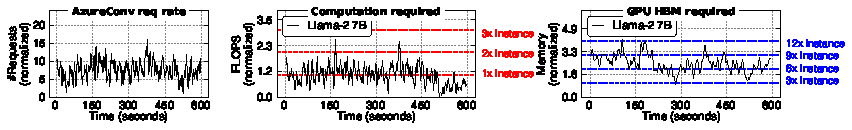
\includegraphics[width=1.01\textwidth,center]{./data/problem/scripts/problem.pdf} \\[0pt]
    \begin{minipage}{1\linewidth}
    \caption{\small{\textit{
        真实 AzureConv~\cite{AzurePublicDataset} 轨迹的请求到达率时间线（a），
        以及在无 SLO 违约条件下服务该工作负载所需的计算资源（b）与内存资源（c）。
    }}}
    \label{fig:problem-statement}
    \end{minipage} \\[-15pt]
\end{figure*}

\begin{figure}[!t]
    \begin{minipage}{1\linewidth}
        \hspace{-1mm}
        \centering
        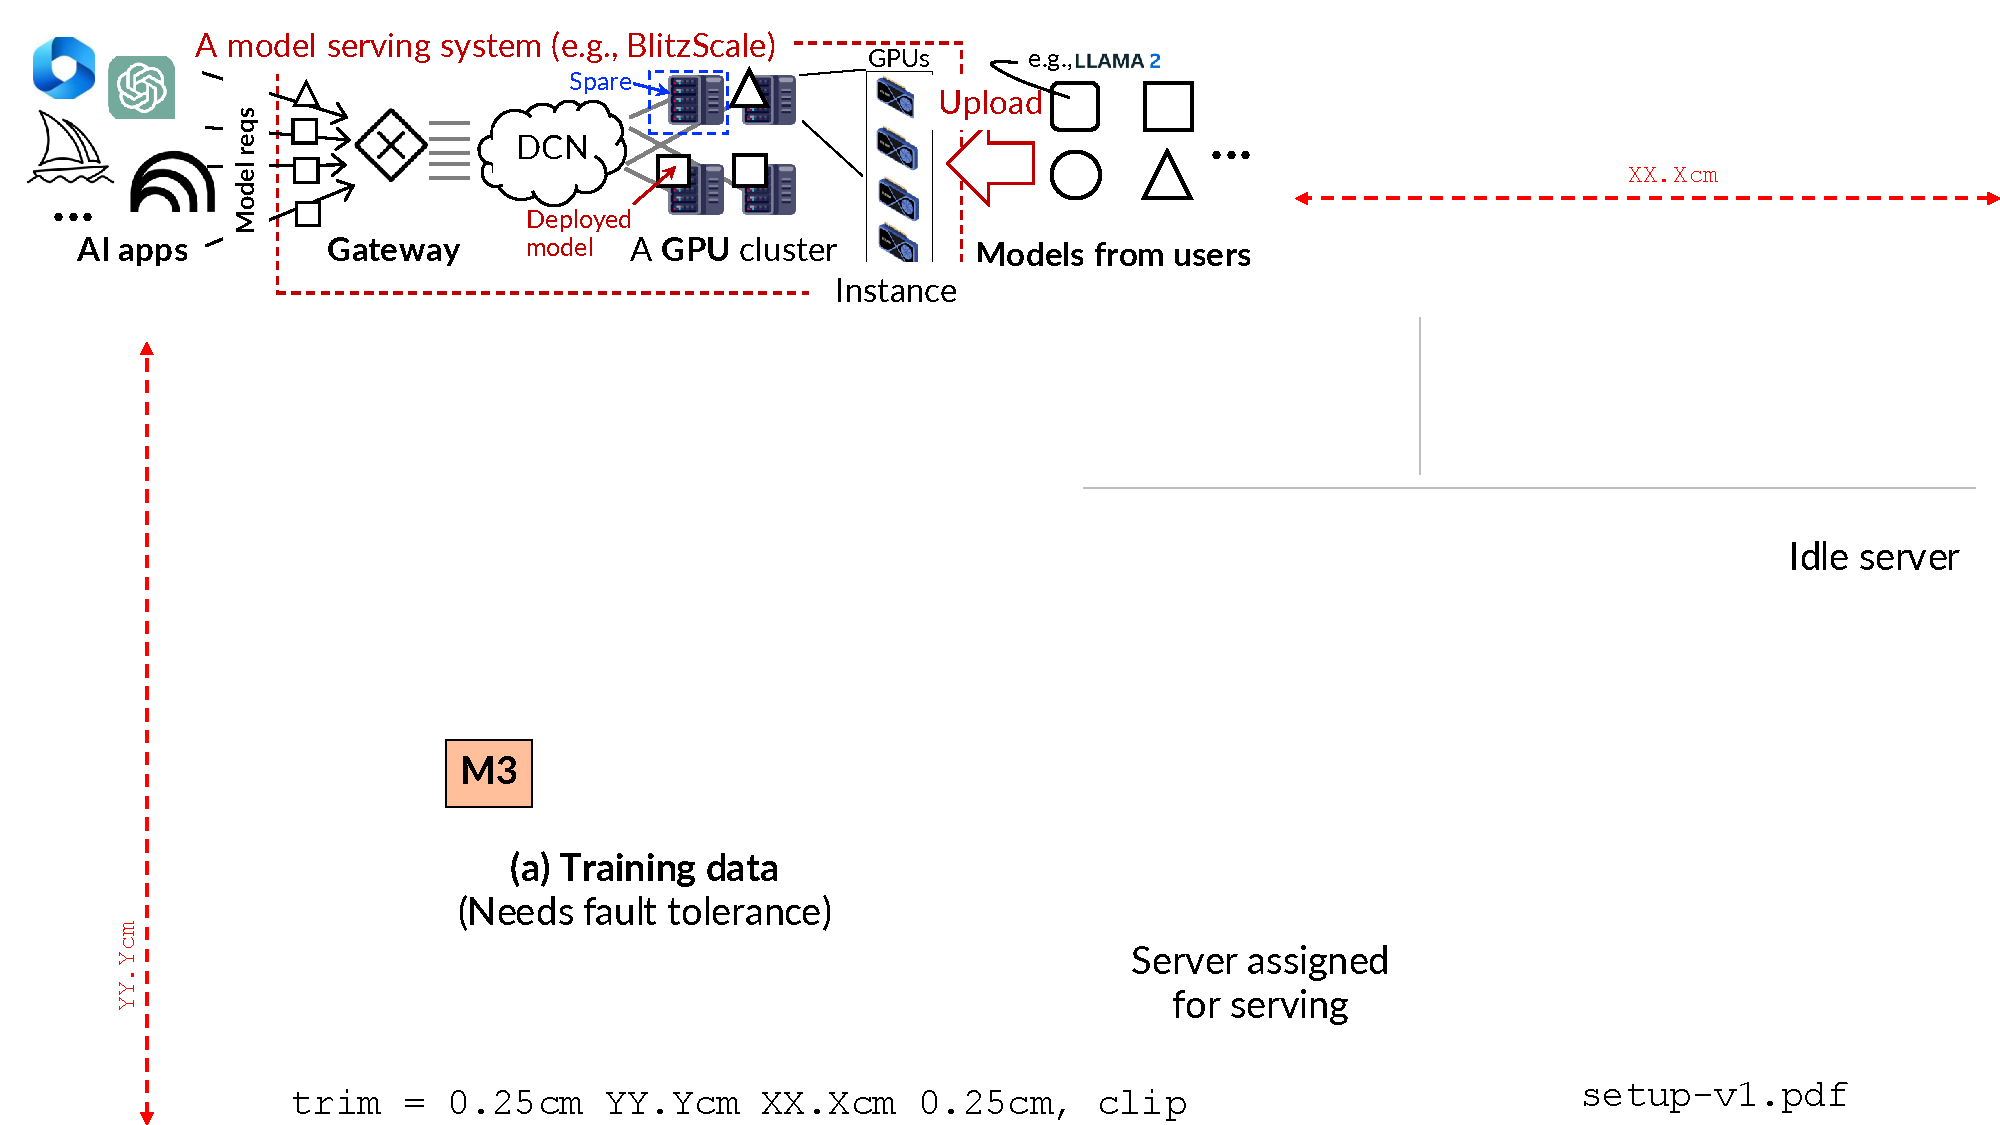
\includegraphics[width=\columnwidth, trim=0.25cm 13.8cm 12cm 0.25cm, clip]{figs/setup-v1.pdf} \\[1pt]
    \end{minipage} \\[3pt]
    \begin{minipage}{1\linewidth}
        \caption{\small{\textit{
            模型即服务（{\maas}）系统示意图。
            其中 DCN 表示数据中心网络（data center network）。
        }}}
        \label{fig:setup}
    \end{minipage} \\[-20pt]
\end{figure}

\nospacestitle{{\maas} 系统设置与服务实例。\,}
{\sys} 面向 {\maas} 场景~\cite{serverless-together-ai,serverless-ray,deepinfra,DBLP:conf/asplos/YangZLZLZCL22,ali-serverless-llm,aws-serverless-llm,DBLP:journals/corr/abs-2401-14351}：
云平台允许用户把模型部署到其托管硬件上进行服务，
并仅按满足 SLO 的请求数量向用户计费~\cite{aws-serverless-llm,ali-serverless-llm}。
这些模型既可以是 Qwen~\cite{qwens} 这样的热门开源模型，
也可以是用户自行上传的定制模型。
得益于这种计费方式，
云平台可以针对特定模型动态调整硬件资源，
以尽可能提高整体硬件利用率。
{\fig{fig:setup}} 展示了一个典型 {\maas} 系统的部署方式。
对于每个用户部署的模型，
系统会动态分配所需的 GPU 资源来处理其推理请求。
需要注意的是，由于 AI 应用种类繁多，
一个 {\maas} 系统往往会同时服务数百甚至数千个模型~\cite{alibailian}。

在本文中，
我们用 \emph{instance} 表示一组 GPU，
它们共同存放模型参数的完整副本，并用于服务该模型。
当模型较小时，一个实例只需要一张 GPU；
当模型较大、参数需要跨多张 GPU 切分时，
一个实例也可能包含多张 GPU，例如采用张量并行~\cite{narayanan2021efficient}。
由于单个实例的服务吞吐存在上限，
云平台通常会为同一个模型部署多个实例，
即分配多组 GPU 共同服务，
并根据请求到达率动态调整实例数量。
{\sys} 能够与现有各种实例级模型服务方法兼容，并为它们提供自动扩缩容支持。

\stitle{实例内服务：非 LLM 与 LLM。\,}
每个服务实例的基本处理流程如下：
它按照逐层计算的方式查询模型（见 {\fig{fig:overview}} (a)），
并最终得到输出结果。
对于视觉模型等简单模型，
用户只需用输入数据（例如图像）查询模型一次即可。
而对于大语言模型（LLM）~\cite{DBLP:conf/nips/VaswaniSPUJGKP17}，
一次请求需要多次查询模型。
模型首先接收输入文本（prompt）并生成第一个结果 token，
这一阶段通常称为 \emph{prefill}。
随后，模型会基于已生成 token 迭代地产生后续 token，
直到返回终止标记；
这个自回归阶段称为 \emph{decode}。

我们强调 LLM 的两个重要特性。
第一，prefill 与 decode 的性能通常分开衡量：
prefill 采用首 token 时间（TTFT）指标，
decode 采用 token 间时间（TBT）指标。
第二，LLM 查询具有状态性：
在请求的自回归阶段，中间结果——通常称为 \emph{KVCache}——会被保存在 GPU 显存中，以加速后续计算。

\stitle{跨实例服务：Prefill/Decode 解耦的 LLM 服务。\,}
观察到 prefill 与 decode 在计算模式上存在明显差异后，
近期工作提出把负责 prefill 与 decode 的实例分离（即 PD disaggregation），
从而处理服务请求~\cite{DBLP:conf/isca/PatelCZSGMB24, DBLP:conf/osdi/ZhongLCHZL0024,DBLP:journals/corr/abs-2401-11181}。
具体而言，对于每个请求，
由一个实例负责 prefill 阶段（prefill instance），
另一个实例负责 decode 阶段（decode instance）。
这种方式需要在两个实例之间搬运大量数据，
因为 prefill 实例必须把 KVCache 传给 decode 实例。
{\sys} 同时支持 PD 解耦和非解耦两类 LLM 服务方式。

\subsection{服务单个模型时的动态硬件需求}
\label{sec:problem-statement}

\noindent
为一个模型确定合适的硬件配置——也就是确定所需实例数量——并不容易，
因为硬件需求既难以预测，又会持续波动。
首先，服务工作负载中的请求到达率会随时间变化，
而且通常难以预测~\cite{DBLP:journals/corr/abs-2401-14351,DBLP:conf/usenix/ShahradFGCBCLTR20,DBLP:conf/nsdi/0025TKS23}。
{\fig{fig:problem-statement}} (a) 展示了真实轨迹中某个单模型服务的请求数时间线——BurstGPT~\cite{wang2024burstgpt}：
在没有明显规律的情况下，
进入系统的推理请求可以在 2 秒内增长 5\,$\times$。
由于单个实例的 FLOPS 是固定的，
这种难以预测的到达率波动会导致所需计算资源——也就是在 SLO 内完成待处理请求所需的 FLOPS——同样变得不可预测。
{\fig{fig:problem-statement}} (b) 通过测量 Llama2-7B 在 BurstGPT 上服务时 prefill 实例的需求，
验证了这一点。

其次，现代模型（尤其是 LLM）服务还会带来复杂且不可预测的显存需求。
如 {\fig{fig:problem-statement}} (c) 所示，
当使用 Llama2-7B 服务 BurstGPT 时，
decode 实例上的 KVCache 占用会达到单个实例显存容量的数倍，
并随时间在 3--12\,$\times$ 之间波动。
根本原因在于，
请求的 KVCache 必须在 decode 阶段常驻于 GPU 显存中。
这些 KVCache 非常大，
例如在 Llama2-7B 服务 BurstGPT 时可达到 190--760\,GB，
而且由于 LLM 的自回归特性，请求在系统中的停留时间也不可预测。
为了避免内存不足带来的性能损失，
{\maas} 系统必须分配足够多的实例来容纳正在执行请求的 KVCache，
因此，一个模型所需的实例数量也会出现不可预测的波动。

\subsection{用于处理动态需求的模型自动扩缩容}

\noindent
模型自动扩缩容会在空闲 GPU 上动态部署\footnote{\footnotesize{系统也会通过停止服务实例来缩容。由于缩容相对简单，本文不再展开。}}
新的服务实例，从而提升服务能力；
这被认为是应对计算与内存需求波动的一个有前景方案~\cite{DBLP:journals/corr/abs-2401-14351,DBLP:conf/asplos/YangZLZLZCL22,serverless-ray}。
其基本逻辑在于：
单个模型的工作负载虽然难以预测，
但平台上所有模型负载叠加后的总体需求通常更平稳~\cite{DBLP:conf/nsdi/0025TKS23}。
因此，当某个模型的服务负载上升时，
系统能够从其他模型那里回收空闲 GPU，
再将其用于扩容该模型。

扩出一个实例通常包含两个基本步骤：
(1) 初始化合适的执行上下文，例如创建 CUDA 上下文（控制平面）；
(2) 把模型参数加载到 GPU 显存中（数据平面）。
本文主要关注步骤 (2)，
因为步骤 (1) 已经可以通过近期 GPU 启动优化方法（例如 checkpoint/restore）~\cite{DBLP:journals/corr/abs-2405-12079,DBLP:conf/asplos/ZengXGCL25}
以及我们基于 Rust/C++ 的服务框架显著压缩（也见 \textsection{\ref{sec:eval-ablation}}）。
对于步骤 (2)，
当前最先进系统 ServerlessLLM~\cite{DBLP:journals/corr/abs-2401-14351}
通过面向 SSD 的参数加载优化了数据平面。
但它并没有从模型服务对扩缩速度的要求出发进行设计。
下一节中的测量结果表明，
基于 SSD 的扩缩速度仍然明显落后于实际应用需求。

\begin{figure*}[!t]
    \centering
    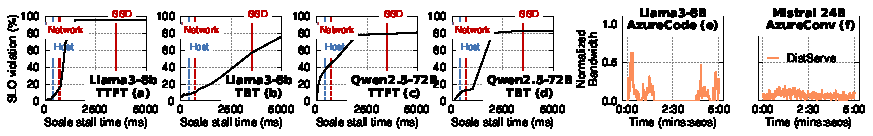
\includegraphics[width=1.01\textwidth,center]{./data/motiv-slo-all.pdf} \\[2pt]
    \begin{minipage}{1\linewidth}
    \caption{\small{\textit{
        在 BurstGPT~\cite{wang2024burstgpt} 上，不同推理场景 (a)--(d) 在不同自动扩缩停顿时间下的 SLO 达成情况；
        (e) 与 (f) 则分析了服务工作负载中的计算网络使用情况。
        评测设置见 \textsection{\ref{sec:eval}}。
    }}}
    \label{fig:motiv-scale-speed}
    \end{minipage} \\[-5pt]
\end{figure*}

\section{实例间扩缩容需求与计算网络特征分析}
\label{sec:bg-motiv}

\nospacestitle{模型自动扩缩容需要快速数据平面。\,}
如果数据平面的速度不够快，
那么在突发期间，
请求仍会因为排队时间变长而违反 SLO。
这里的 SLO 指的是端到端时延约束，
即从请求发出到推理结果返回的总耗时。
因此，这一时延自然也包含了等待新扩出实例就绪所产生的排队延迟。

为了刻画不同扩缩速度对 SLO 达成率的影响，
我们在 DistServe~\cite{DBLP:conf/osdi/ZhongLCHZL0024} 上实现了一个模拟器：
该模拟器把模型预先部署到所有 GPU 上，
然后通过人为插入延迟来模拟不同的数据平面速度。
TTFT 与 TBT 的 SLO 设置遵循已有工作~\cite{DBLP:conf/osdi/ZhongLCHZL0024} 中不同模型的推理速度。
具体来说，
对于 Llama3-8B，我们采用 450\,ms 的 TTFT SLO 和 150\,ms 的 TBT SLO；
对于张量并行度为 4 的 Qwen2.5-72B，我们采用 1250\,ms 的 TTFT SLO 和 200\,ms 的 TBT SLO。
更详细的评测设置见 \textsection{\ref{sec:eval}}。

{\fig{fig:motiv-scale-speed}} (a)--(d) 展示了结果。
可以看到，
对于 72\,B 模型，
若想把 SLO 违约率控制在 60\,\% 以下，
单个实例、每张 GPU 至少需要 220\,Gbps 的扩缩速度\footnote{\footnotesize{72\,B 模型的单个实例使用 4 张 GPU。}}；
而这一速度只有在模型参数从主机内存加载时才能达到。
扩缩时间需求与推理时间直接相关——我们评测的 BurstGPT~\cite{wang2024burstgpt}
工作负载平均 TTFT（含排队）为 771\,ms。
因此，如果要让所有请求都满足 1250\,ms SLO，
扩缩时间必须低于 500\,ms，
也就要求每张 GPU 具备 576\,Gbps 的网络速度
（通过参数规模除以扩缩时间得到）。
这一要求远超厂商提供的每 GPU SSD 带宽（2--10\,Gbps~\cite{googleinstance,awsinstance,volcanoinstance}；详见 \textsection{\ref{sec:appendix-hardware}}）。

\begin{figure}[!t]
    \centering
    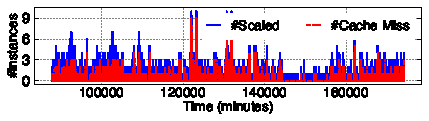
\includegraphics[width=1.01\linewidth,center]{./data/motiv-cache-miss.pdf} \\[1pt]
    \begin{minipage}{1\linewidth}
    \caption{\textit{\small{
        在 BurstGPT~\cite{wang2024burstgpt} 上运行 ServerlessLLM~\cite{DBLP:journals/corr/abs-2401-14351} 时主机缓存未命中的分析。
    }}}
    \label{fig:motiv-cache-miss}
    \end{minipage} \\[-5pt]
\end{figure}

\stitle{从主机内存加载模型参数并不总是有效，因为未命中很常见。\,}
当 CPU 主机内存中缓存了参数时，
借助高速 Host-GPU 互连（例如 256\,Gbps PCIe 4.0），
某些配置（如 8\,B、24\,B）确实能够满足扩缩速度要求。
但是在真实轨迹中，缓存未命中非常常见，
因为有限的主机内存无法支持把 {\maas} 系统中部署的所有模型都缓存下来。
{\fig{fig:motiv-cache-miss}} 展示了在 BurstGPT 工作负载下使用 ServerlessLLM~\cite{DBLP:journals/corr/abs-2401-14351} 时，
扩出的实例数量以及遭遇的缓存未命中情况。
按照其原始设置，
我们将主机缓存的 keep-alive 时间设置为 5 分钟。
可以看到，缓存未命中率会随时间在 20--46\,\% 之间波动，
与 ServerlessLLM 论文中报告的 25--60\,\% 基本一致。
有趣的是，许多未命中发生在需要同时扩多个实例时，
因为涉及主机越多，
在没有缓存该模型参数的主机上扩容的概率就越高。
因此，即使主机缓存未命中，
我们仍然需要找到办法加快扩缩速度。

\begin{figure}[!t]
    \begin{minipage}{1\linewidth}
        \hspace{-1mm}
        \centering
        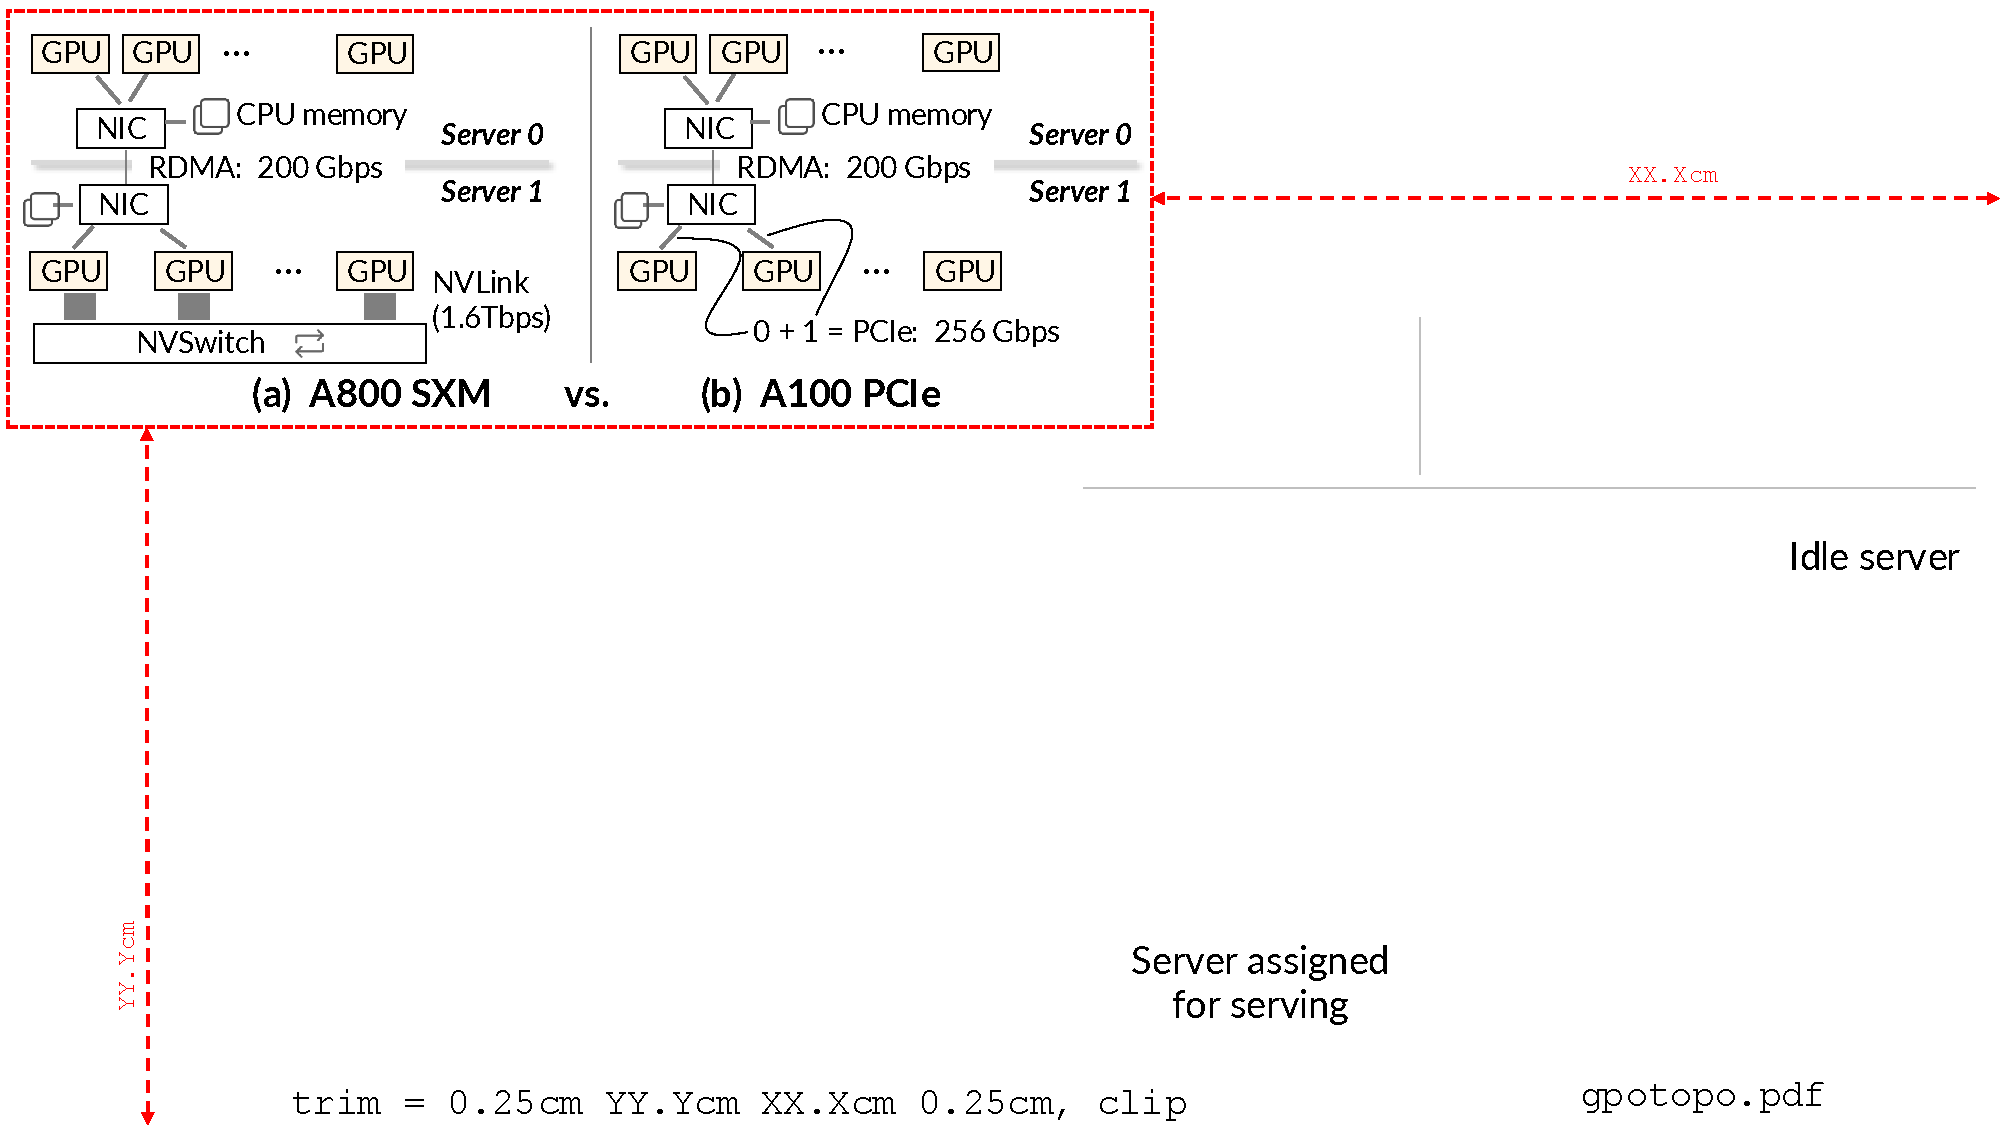
\includegraphics[width=.99\textwidth, trim=0.25cm 11.9cm 14.4cm 0.25cm, clip]{figs/gputopo.pdf} \\[1pt]
    \end{minipage} \\[4pt]
    \begin{minipage}{1\linewidth}
        \caption{\textit{\small{
            带 NVLink（a）与不带 NVLink（b）时，{\maas} 中网络连接方式的示意图。
            注意，一条 256\,Gbps 的 PCIe 链路会被其连接的两张 GPU 共享~\cite{nvidia-all-to-all}。
        }}}
        \label{fig:gputopo}
    \end{minipage} \\[-10pt]
\end{figure}

\stitle{机会：高速且低利用率的计算网络。\,}
首先，GPU（以及 CPU）之间的计算网络速度可与 Host-to-GPU 链路相当，甚至更快。
如 {\fig{fig:gputopo}} 所示，
GPU 间网络（RDMA）的速率可达 200\,Gbps，
已经接近 Host-GPU PCIe 的 256\,Gbps；
而在有 NVLink 时，速度则更高。
更重要的是，
这些网络在服务过程中通常没有被充分利用。
{\fig{fig:motiv-scale-speed}} (e) 与 (f) 测量了 DistServe~\cite{DBLP:conf/osdi/ZhongLCHZL0024} 的峰值网络使用情况。
DistServe 是一个采用 PD 解耦的服务系统，
由于需要搬运 KVCache，因此本身就高度依赖网络。
为了测量峰值用量，
我们把所有 GPU 都用于服务，
并在集群可承受的最大请求率下执行工作负载。
结果表明，即使在峰值负载下，
仍有超过 40\,\% 的网络容量处于空闲状态，
这为利用计算网络承载扩缩容数据平面提供了机会。
